\documentclass[xcolor=svgnames]{beamer}

\usetheme{umbc1} 
%\usecolortheme{default}

\usepackage{../mystyle}
\usepackage{multicol}
\usepackage{verbatim}
\usepackage{capt-of}
\usepackage{natbib}
\usepackage{url}
\usepackage{hyperref}
\hypersetup{colorlinks,linkcolor=,urlcolor=Blue}

% keep only the style and the slide number in the footer:
\setbeamertemplate{footline}[text line]{%
  \vbox{%
    \insertvrule{2.0pt}{umbc@decorations.fg!50!bg}%
    \begin{beamercolorbox}[wd=\paperwidth,ht=2.25ex,dp=1ex]{umbc@decorations}%
            \Tiny\hspace*{4.65in}\insertframenumber{} %/ \inserttotalframenumber\hspace*{2ex}\hspace{4mm}
    \end{beamercolorbox}}}


%\beamertemplatenavigationsymbolsempty
%\setbeamertemplate{footline}[frame number]

\title{~\\~\\Geostatistical inference under preferential sampling: Final presentation
\\
{\small By Peter Diggle, Raquel Menezes, and Ting-li Su}
}
\author[John Paige]{John Paige}
\date[\today]{\vspace{.3in} \small \\ \today}
\institute[University of Washington] % (optional, but mostly needed)
{
  \vspace{.1in} \\ Statistics Department\\
{\sc  University of Washington  }
}

\begin{document}
\setlength{\columnsep}{.5cm}


\frame{\titlepage}

%---------------------------------------------------------------------------------------------------------------------------------------

%\begin{frame}
 % \frametitle{Outline}
 % \tableofcontents
%\end{frame}


%----------------------------------------------------------------------------------------------------------------------------------------
%  Section 1
%----------------------------------------------------------------------------------------------------------------------------------------
\section{Introduction}

%\begin{frame}
%  \frametitle{Outline}
%  \tableofcontents[currentsection]
%\end{frame}

%\frame{\tableofcontents}

%\subsection{Introduction to Problem}

%----------------------------------------------------------------------------------------------------------------------------------------
\begin{frame}
\frametitle{Divisions of Spatial Statistics}

\begin{columns}

\column{2.5in}
\begin{itemize}
\item \citet{Cressie1991} and \citet{gelfand2010} divide spatial statistics into 3 areas:
\begin{itemize}
\item \alert<1>{discrete data}
\item \alert<2>{continuous data}
\item \alert<3>{point patterns}
\end{itemize}
\end{itemize}

\uncover<4>{
\begin{itemize}
\item \citet{diggle2013} instead gives 2 subdivisions of spatial statistics:
\begin{itemize}
\item continuous data
\item discrete data
\end{itemize}
\item This emphasizes random nature of sampling locations
\end{itemize}
}

\column{2.5in}
\begin{center}
\includegraphics[width=2.2in]<2>{continuousData.pdf}
\includegraphics[width=2.2in]<1>{discreteData.pdf}
\includegraphics[width=2.2in]<3>{PPData.pdf}
\includegraphics[width=2.2in]<4>{GPPPData.pdf}
\end{center}

\end{columns}

\end{frame}
%----------------------------------------------------------------------------------------------------------------------------------------
\begin{frame}
\frametitle{Divisions of Spatial Statistics}

\begin{columns}

\column{2.5in}
\begin{itemize}
\setlength\itemsep{.15in}
\item Classically, data locations are assumed to be fixed constants
\item What happens when the sample locations depend on the measured process itself?
\begin{itemize}
\item This is called \tbf{preferential sampling}
\end{itemize}
\end{itemize}

\column{2.5in}
\begin{center}
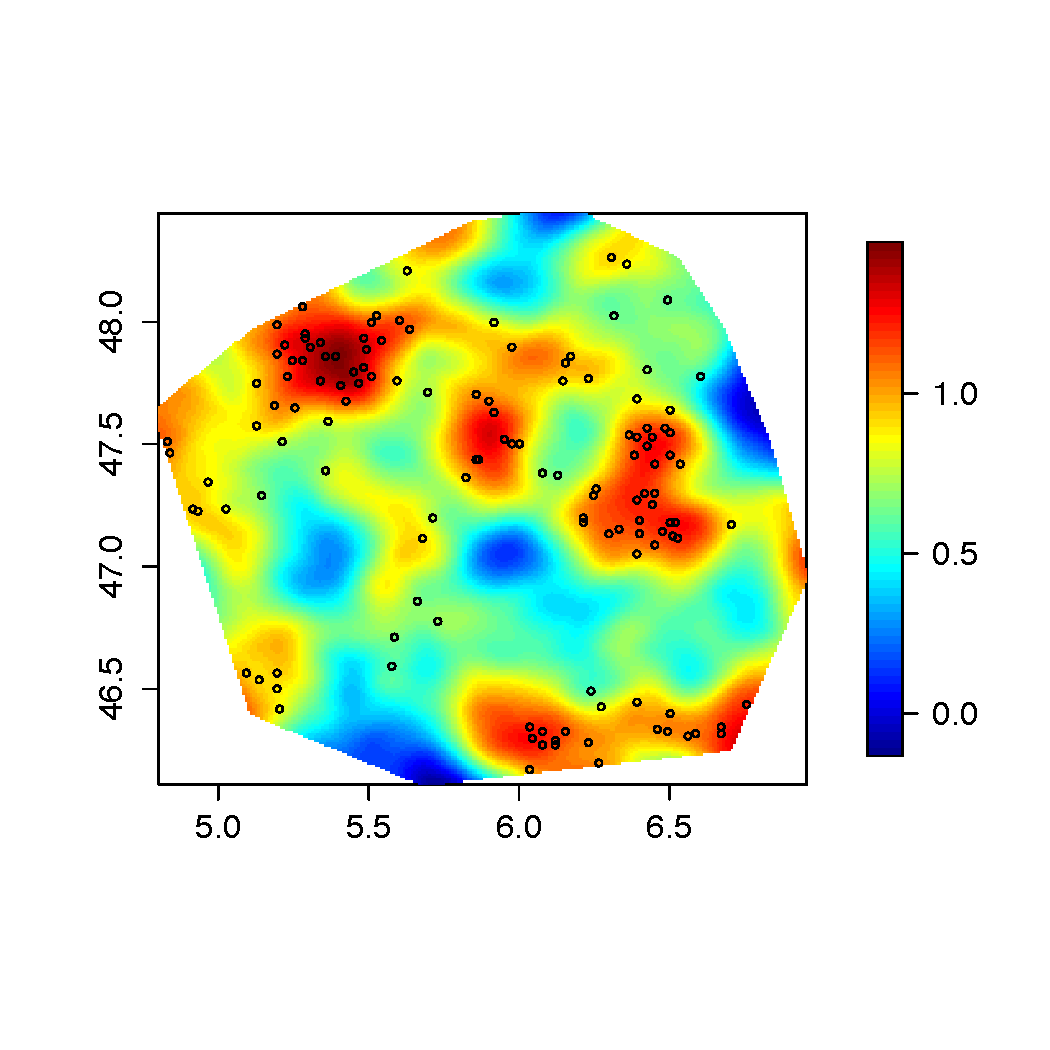
\includegraphics[width=2.2in]{GPPPData.pdf}
\end{center}

\end{columns}

\end{frame}
%----------------------------------------------------------------------------------------------------------------------------------------
\begin{frame}
\frametitle{Problems Addressed}
\begin{columns}

\column{2.5in}
\begin{itemize}
\setlength\itemsep{.15in}
\item Determining if data is sampled preferentially
\item How preferential sampling affects `naive' inference
\item Effective model for preferential sampling
\item Focus on lead levels in Galicia, Spain and simulated experiments
\end{itemize}

\column{2.5in}
\begin{figure}
\centering
\image{width=2.5in}{sampling_locations.pdf}
\end{figure}

\end{columns}

\end{frame}

%----------------------------------------------------------------------------------------------------------------------------------------
\begin{frame}
\frametitle{Classical Model}

$$ Y_i = \mu + S(x_i) + Z_i, $$
$Y_i$: observation at location $x_i$\\
$\mu$: mean\\
$S(\v{x}) \sim \MVN{\v{0}, \Sigma(\v{x})}$: spatially correlated portion of process\\
$Z_i \iid \Norm{0, \tau^2}$: measurement noise\\
\uncover<2->{
$\Rightarrow$ $\v{Y} \sim \MVN{\v{\mu}, \Sigma_0}$, where $\Sigma_0 = \Sigma_0(\v{\theta}) = \Sigma + \tau^2I$}\\~\\
\uncover<3->{
Log likelihood:
$$\mcal{L}(\v{\theta}) = -\frac{1}{2}\log(|\Sigma_0|) - \frac{1}{2}(\v{Y} - \v{\mu})' \Sigma_0^{-1} (\v{Y} - \v{\mu}) - \frac{n}{2}\log(2\pi)$$
}
\end{frame}
%----------------------------------------------------------------------------------------------------------------------------------------
\begin{frame}
\frametitle{Classical Model}

$$ Y_i = \mu + S(x_i) + Z_i, $$
$Y_i$: observation at location $x_i$\\
$\mu$: mean\\
$S(\v{x}) \sim \MVN{\v{0}, \Sigma(\v{x})}$: spatially correlated portion of process\\
$Z_i \iid \Norm{0, \tau^2}$: measurement noise
\\~\\
Common assumptions:
\begin{itemize}
\item $x_i$ are sampled independently of true process $\mu + S$
\item Stationarity
\end{itemize}

\end{frame}
%----------------------------------------------------------------------------------------------------------------------------------------
\begin{frame}
\frametitle{Variograms}

\begin{itemize}
\setlength\itemsep{.05in}
\item \tbf{Stationarity}: under stationarity, $\var{S(x_i) - S(x_j)} = V(x_i - x_j)$
\item \tbf{Isotropy}: under isotropy (and stationarity), $\var{S(x_i) - S(x_j)} = V(|x_i - x_j|)$
\item \tbf{Variograms} define the spatial structure of the covariance in $S$
\item Empirical estimate given data $Y_i$ at location $x_i$ (under stationarity and isotropy):
$$ \wh{V}(d) = \frac{1}{| N(d)|} \sum_{|x_i - x_j| \in N(d)} (Y_i - Y_j)^2 $$
where $N(d)$ is the set of pairs $(x_i,x_j)$ with $|x_i - x_j| \approx d$
\item This estimator assumes non-preferentiality
\end{itemize}

\end{frame}
%----------------------------------------------------------------------------------------------------------------------------------------
\begin{frame}
\frametitle{Variograms}

Mat\'{e}rn theoretical variogram:
$$ V(d) = \sigma^2(1- \rho(u \ \vert \ \phi, \kappa)) + \tau^2$$
where
$$\rho(u \ \vert \ \phi, \kappa) = \frac{1}{2^{\kappa - 1} \Gamma(\kappa)} (u/\phi)^{\kappa} K_\kappa(u/\phi), $$
is the Mat\'{e}rn correlation function\\~\\
$u$: distance\\
$\phi$: scale\\
$\kappa$: smoothness\\
$\sigma^2$: is the variance of $S$\\
$\tau^2$: measurement variance\\
$K_\kappa(\cdot)$: Bessel function

\end{frame}
%----------------------------------------------------------------------------------------------------------------------------------------
\begin{frame}
\frametitle{Variograms of Log-Lead Data (Classical)}

\image{width=2.22in}{vario97.pdf} \image{width=2in}{vario00.pdf}

\end{frame}
%----------------------------------------------------------------------------------------------------------------------------------------
\begin{frame}
\frametitle{Model for Preferential Sampling}

Three assumptions for model:
\begin{enumerate}
\item $S$ is still a stationary, mean zero Gaussian process \\
(so $S(\v{x}) \sim \MVN{\v{0}, \Sigma(\v{x})}$)
\item Conditional on $S$, $X$ is an inhomogeneous Poisson process wtih random intensity
$$\Lambda(x) = \exp{\alpha + \beta S(x)}$$
\item $Y_i \vert S, X \iid \Norm{\mu + S(x_i), \tau^2}$
\end{enumerate}
~\\
1 + 2 $\Leftrightarrow$ $X$ is a log Gaussian Cox process (LGCP)

\end{frame}
%----------------------------------------------------------------------------------------------------------------------------------------
\begin{frame}
\frametitle{Log-Gaussian Cox Processes}

\begin{columns}[l]

\column{.05in}
\column{2.45in}
A \tbf{Cox process} is a stochastic point process that for $B, B'$ bounded Borel sets satisfies:
\begin{itemize}
\item $N(B)~\sim~\Pois{\int_B \Lambda(x) \ dx}$
\item $N(B) \indep N(B')$ when $B \cap B' = \emptyset$
\end{itemize}

\column{2.45in}

\begin{figure}
\centering
\image{width=2.45in}{cox_proc_fig.pdf}
\caption{From \citealt{diggle2010}.  An example of a LGCP on unit square where $\beta=2$, $\alpha=1$, and $S$ has Mat\'{e}rn covariance.}
\end{figure}

\column{.05in}

\end{columns}

\end{frame}
%----------------------------------------------------------------------------------------------------------------------------------------
\begin{frame}
\frametitle{Testing Affect of Sample Designs: Samplings Schemes}
\begin{figure}
\centering
\image{width=4.5in}{sim_design.pdf}
\caption{From \citealt{diggle2010}}
\end{figure}
Variogram estimation tested under 500 simulations from three sampling designs:
\begin{enumerate}
\item[a] Uniform
\item[b] Preferential ($\beta=2$)
\item[c] Clustered
\end{enumerate}

\end{frame}
%----------------------------------------------------------------------------------------------------------------------------------------
\begin{frame}
\frametitle{Classical Variogram Bias Under Preferential Sampling}
\begin{figure}
\centering
\vspace{-.0in}
\image{width=4.0in}{VGbias.pdf}
\vspace{-.0in}
\caption{Variogram bias $\pm$2 standard errors and standard deviations for uniform (solid), clustered (dashed), and preferential (dotted) sampling schemes.}
\end{figure}

\end{frame}
%----------------------------------------------------------------------------------------------------------------------------------------
\begin{frame}
\frametitle{Classical Prediction Bias Under Preferential Sampling}
\begin{table}[ht]
\centering
\begin{tabular}{|r|cccc|}
\hline
\emph{Mod.} &  \emph{Param.} &  \multicolumn{3}{c|}{\emph{Confidence intervals}}  \\ \cline{3-5}
& & \emph{Uniform} & \emph{Preferential} & \emph{Clustered} \\
\hline
1 & Bias & (-0.029,  0.038) & (0.956, 1.123) & (-0.074, 0.064) \\ 
1 & RMSE & (0.354, 0.410) & (1.318, 1.501) & (0.717, 0.851) \\ 
2 & Bias & (-0.040,  0.030) & (-0.265, -0.195) & (-0.040, 0.032) \\
2 & RMSE & (0.375, 0.425) & (0.434, 0.491)& (0.382, 0.432) \\
\hline
\end{tabular}
\caption{Classical predictions using 95\% Confidence intervals for the given parameters under the given models and sampling schemes}
\end{table}
Models:
\begin{enumerate}
\item $(\mu=4, \sigma^2=1.5, \phi=.15, \kappa=1, \beta=2)$
\item $(\mu=1.51, \sigma^2=.14, \phi=.31, \kappa=.5, \beta=-2.20, \tau^2=.059)$
\end{enumerate}

\end{frame}
%----------------------------------------------------------------------------------------------------------------------------------------
\begin{frame}
\frametitle{Preferential Model Likelihood}
Make gridded approximation of $S = \{S_0, S_1\}$ on lattice $X^* = \set{x_1^*, ..., x_N^*}$.
\begin{itemize}
\item $S_0$ are data
\item $S_1$ are the values at other grid points
\end{itemize}
\bal
L(\vt) &= \int \pi(Y \vert X, S) \pi(X \vert S) \pi(S) \ dS \\
&= \hdots \\
%&= \int \pi(X \vert S) \pi(Y \vert X, S) \frac{\pi(S \vert Y)}{\pi(S \vert Y)} \pi(S) \ dS \\
%&= \int \pi(X \vert S) \pi(Y \vert S_0) \frac{\pi(S \vert Y)}{\pi(S_0 \vert Y) \pi(S_1 \vert S_0, Y)} \pi(S) \ dS \\
%&= \int \pi(X \vert S) \pi(Y \vert S_0) \frac{\pi(S \vert Y)}{\pi(S_0 \vert Y) \pi(S_1 \vert S_0)} \pi(S_0, S_1) \ dS \\
%&= \int \pi(X \vert S) \pi(Y \vert S_0) \frac{\pi(S \vert Y)}{\pi(S_0 \vert Y)} \pi(S_0) \ dS \\
&= E_{S \vert Y} \brack{\pi(X \vert S) \frac{\pi(Y \vert S_0)}{\pi(S_0 \vert Y)} \pi(S_0)} \\
&\approx m^{-1} \sum_{j=1}^m \pi(X \vert S_j) \frac{\pi(Y \vert S_{0j})}{\pi(S_{0j} \vert Y)} \pi(S_{0j})
\eal
where $S_j$ is the $j$th conditional simulation of $S$ conditioned on $Y$.
\end{frame}
%----------------------------------------------------------------------------------------------------------------------------------------
\begin{frame}
\frametitle{Preferential Model Likelihood}
Define $C$ as a $n \times N$ matrix with a single 1 in each row and all else 0 s.t. $X = C X^*$.
\\~\\
Steps for Monte Carlo Simulation:
\begin{enumerate}
\item Simulate $\v{S} \sim \MVN{\v{0}, \Sigma}$ using Circulant Embedding \citep{woodChan1994}
\item Compute $j$th simulation of $\v{S} \vert \v{Y}$:
$$ \v{S}_j \defn \v{S} + \Sigma C' \Sigma_0^{-1}(\v{Y} - \v{\mu} + \v{Z} - C \v{S}) $$
Where $Z_i \iid \Norm{0, \tau^2}$
\item Calculate $m^{-1} \sum_{j=1}^m \pi(X \vert \v{S}_j) \frac{\pi(\v{Y} \vert \v{S}_{0j})}{\pi(\v{S}_{0j} \vert \v{Y})} \pi(\v{S}_{0j})$
\end{enumerate}
\end{frame}
%----------------------------------------------------------------------------------------------------------------------------------------
\begin{frame}
\frametitle{Preferential Model Likelihood}
\bal
\pi(X \vert \v{S}_j) &= \paren{\prodi \Lambda(x_i)} \paren{\int \Lambda(x) \ dx}^{-n}\\
\v{Y} \vert \v{S}_{0j} &\sim \MVN{ \v{S}_{0j}, \tau^2 I} \\
\v{S}_{0j} \vert \v{Y}  &\sim \MVN{\Sigma C' \Sigma_0^{-1}(\v{Y} - \v{\mu}), \Sigma - \Sigma C' \Sigma_0^{-1} C \Sigma}  \\
\v{S}_{0j} &\sim \MVN{\v{0}, C \Sigma C'} 
\eal
\end{frame}
%----------------------------------------------------------------------------------------------------------------------------------------
\begin{frame}
\frametitle{Goodness of Fit}
\emph{Reduced second moment measure} (or $K$-function) for defined model is given by:
$$ K(s) = \pi s^2 + 2 \pi \int_0^s (\exp{\beta^2 \sigma^2 \rho(u; \kappa, \phi)} - 1) u \ du $$
$s$: distance\\
$\rho(u ; \phi, \kappa)$: Mat\'{e}rn correlation function\\~\\
$K$-functions commonly used in goodness of fit tests
\end{frame}
%----------------------------------------------------------------------------------------------------------------------------------------
\begin{frame}
\frametitle{Goodness of Fit: Monte Carlo Testing}
For any Monte Carlo test statistic, $T$, where higher $T$ casts doubt on $H_0$, assume:
\begin{itemize}
\item $T_1$ is from data
\item  $T_2, ..., T_{n}$ are simulated under $H_0$
\end{itemize}
Then our $p$-value is the rank of $T_1$ out of $T_1, T_2, ..., T_n$ (\emph{i.e.} if $n=100$ and $T_1$ is largest test statistic, $p=.01$).
\end{frame}
%----------------------------------------------------------------------------------------------------------------------------------------
\begin{frame}
\frametitle{Goodness of Fit: Monte Carlo Testing}
\begin{figure}
\centering
\image{width=4in}{envelope.pdf}
\end{figure}
$p=0.07$
\end{frame}
%----------------------------------------------------------------------------------------------------------------------------------------
\begin{frame}
\frametitle{Problems with the Methodology}
\begin{itemize}
\item No cross-validation performed (effectiveness of $K$-function goodness of fit tests unclear)
\item Predictive distribution assumes non-preferentiality with plug-in parameters from preferential model
\item Predictive distribution has unreasonable certainty in locations far from data
\item Joint non-preferential model gives parameters similar to preferential model parameters:
\begin{itemize}
\item My non-preferential model: \\
$(\h{\mu}_{97} = 1.551, \h{\mu}_{00} = 0.727, \h{\sigma}^2=0.136, \h{\phi}=0.305, \h{\tau}^2=0.052)$
\item Their preferential model: \\
$(\h{\mu}_{97} = 1.515, \h{\mu}_{00} = 0.762, \h{\sigma}^2=0.138, \h{\phi}=0.313, \h{\tau}^2=0.059)$
\end{itemize}
\end{itemize}
\end{frame}
%----------------------------------------------------------------------------------------------------------------------------------------
\begin{frame}
\frametitle{Conclusions}
\begin{itemize}
\item For preferential simulations, variograms estimated naively were biased
\item Uniform sampling performed best, then clustered, then preferential
\item Proposed class of models is flexible and values for $\beta$ can be tested directly with likelihood ratio test
\item LGCP isn't necessarily the best fit for the log-lead data
\item LGCP model gives tractable Monte Carlo likelihood
\item LGCP model has easy goodness of fit tests
\end{itemize}
\end{frame}
%----------------------------------------------------------------------------------------------------------------------------------------

%----------------------------------------------------------------------------------------------------------------------------------------
%  Section 6
%----------------------------------------------------------------------------------------------------------------------------------------
\section{References}
\begin{frame}
\tiny
\frametitle{References}
\bibliographystyle{../te}
\bibliography{../prelim}
\end{frame}
%---------------------------------------------------------------------------------------------------------------------------------------



\end{document}








